%\subsection{Learning of Weights Given Gates: Refining and Extending Prior Work}\label{sec:analysis}

%In what follows, we first restate the prior result. While \Cref{th:fc} and Theorem 5.1 in \citep{npk} are mathematically identical, \Cref{th:fc} is written in a manner to capture the fact that the NPK is invariant to permutation of the layers. \Cref{th:conv,th:res} are entirely new and are extensions of the dual view for convolutions with global pooling and skip connections. 

\subsection{Theorem Statements}
%\subsection{NPK of FC-DNN: Product Kernel }
%\input{cnpkexample}
%\subsection{Neural Path Kernel : Similarity based on active sub-networks}
%\textbf{Remark.} In the case of fully connected networks, $\textbf{overlap}_{\Theta}(i,x,x')$ is equal for all $i\in[\din]$, and hence $\text{NPK}_{\Theta}(x,x')=\ip{x,x'}\cdot\textbf{overlap}_{\Theta}(x,x')$.
%We point out that this statistical decoupling of weights and gates in \Cref{assmp:main} is unrealisable in a DNN with ReLU, however, this assumption can be trivially realised in a DGN. %Further, we are interested only in the `what?' ( and not `how?') question related to the gates in which case this assumptions is not a restriction.

\begin{theorem}[Product of Kernels Theorem]
\label{th:fc} Under \Cref{assmp:main}  ($\sigma=\frac{\cscale}{\sqrt{w}}$) for FC-DGN : 
\begin{align*}
\text{NTK}_{\text{DGN}}(x,x') \rightarrow d \cdot \cscale^{2(d-1)} \cdot \left(\ip{ x,x'} \cdot \Pi_{l=1}^{d-1} \frac{\ip{G_l(x),G_l(x')}}w\right), \quad\text{as}\,\, w\rightarrow \infty 
\end{align*}
\end{theorem} 
%\textbf{Remark.} Here $\frac{\ip{G_l(x),G_l(x')}}w$ are the \emph{base kernels} measuring the \emph{\textbf{correlation of the gates}}. We show experimentally that the correlation of gates is essentially  `what is learnt in a DNN with ReLUs'.
%and $\Pi_{l=1}^{d-1} \frac{\ip{G_l(x),G_l(x')}}w$ is a product of these base kernels and hence the name `Product of Kernels Theorem'.  The base kernels are essentially measuring which we show via  We now list the roles of the two networks, weights, depth and width.

%\textbf{Feature Network.} The role of this network is to process the input layer-by-layer and produce the $w$-dimensional gating features $G_l(\cdot)$. Each layer comprises of `$w$' ReLUs, and a given ReLU (i.e., gate) is `on' if the input to that layer lies on the positive half-space of hyperplane of given by the incoming weights of that ReLU. Thus the gates of a given layer are based on the angle between the input to that layer and the various hyperplanes given by the weights of that layer. Prior experiments in [\citenum{npk}] and the experiments in this paper show that the feature network, i.e., the gates hold most information, which in turn means that weights of the feature network are key.

%\textbf{Value Network}. The value network implements the product of kernels by laying out the gates as masks depth-wise, and connecting them in the structure of a DNN. Note that depth-wise layout plays an important role here: for instance, if we were to concatenate the gating features as $\varphi(x)=(G_l(x),l=1,\ldots,d-1)\in\{0,1\}^{(d-1)w}$, it would have only resulted in the kernel $\ip{\varphi(x),\varphi(x')}=\sum_{l=1}^{d-1}{\ip{G_l(x),G_l(x')}}$, i.e., a \emph{sum  (not product)} of kernels. Prior experiments in [\citenum{npk}] and the experiments in this paper show that the value network can be reset and re-trained without loss of performance, which in turn means that weights of the value network are not that important.

%\textbf{Note.} The above insights from \Cref{th:main} carry over to the case of DNN with ReLUs by thinking that the roles of value and feature network are performed by a single network.

\textbf{Convolutions with pooling.} Let the circular rotation of vector $x\in\R^{\din}$ by `$r$' co-ordinates be defined as $rot(x,r)(i)=x(i+ r)$, if $i+r \leq \din$ and $rot(x,r)(i)=x(i+ r-\din)$ if $i+r > \din$. Using circular convolutions with pooling results in a rotationally invariant kernel \Cref{th:mainconv}. The architecture and the notations for the network with convolutions is presented in the Appendix.
\begin{comment}
 We extend the dual view to neural network with $\dc$ convolutional layers ($l=1,\ldots,\dc$), followed by a \emph{global-average/max-pooling} layer ($l=\dc+1$) and $\dfc$ ($l=\dc+2,\ldots,\dc+\dfc+1$) fully connected  layers (see Appendix for notation). The convolutional window size is $\wconv<\din$, the number of filters per convolutional layer as well as the width of the fully connected layers is $w$. The main steps are (i) treating pooling layers like gates/masks, (ii) bundling together the paths that share the same path value (due to weight sharing in convolutions) and (iii) re-defining the NPF and NPV for these bundles. The important consequence of weight sharing (due to convolutions and pooling) is that the NPK becomes rotationally invariant resulting in \Cref{th:mainconv}.
\end{comment}
\begin{theorem}[Rotationally Invariant Kernel Theorem]\label{th:conv} Under \Cref{assmp:main}, for  a suitable $\bcnn$:
\begin{align*}
&\kv_{\Tdgn_0}&\ra&\quad \frac{\bcnn}{{\din}^2} \cdot \sum_{r=0}^{\din-1} \ip{x,rot(x',r)}_{\Lambda(\cdot, x,rot(x',r))},\,\, \text{as}\,\,  w\ra\infty\,\text{(for global-average-pooling)}, \\
&\kv_{\Tdgn_0}&\ra& \quad{\bcnn} \cdot \sum_{r=0}^{\din-1} \ip{x,rot(x',r)}_{\Lambda(\cdot, x,rot(x',r))},\,\, \text{as}\,\,  w\ra\infty\,\text{(for global-max-pooling)}
\end{align*}
\end{theorem}

\textbf{Residual Networks with Skip connections.} We consider a ResNet with `$(b+2)$' blocks and `$b$' skip connections between the blocks (left of \Cref{fig:resnet}). Each block is a fully connected (FC) DNN of depth `$\dblock$' and width `$w$'. There are $2^b$ many sub-FC-DNNs within this ResNet (see \Cref{def:subfcdnn} and right of \Cref{fig:resnet}).
%\FloatBarrier
\begin{figure}[t]
\begin{minipage}{0.5\columnwidth}
\resizebox{\columnwidth}{!}{
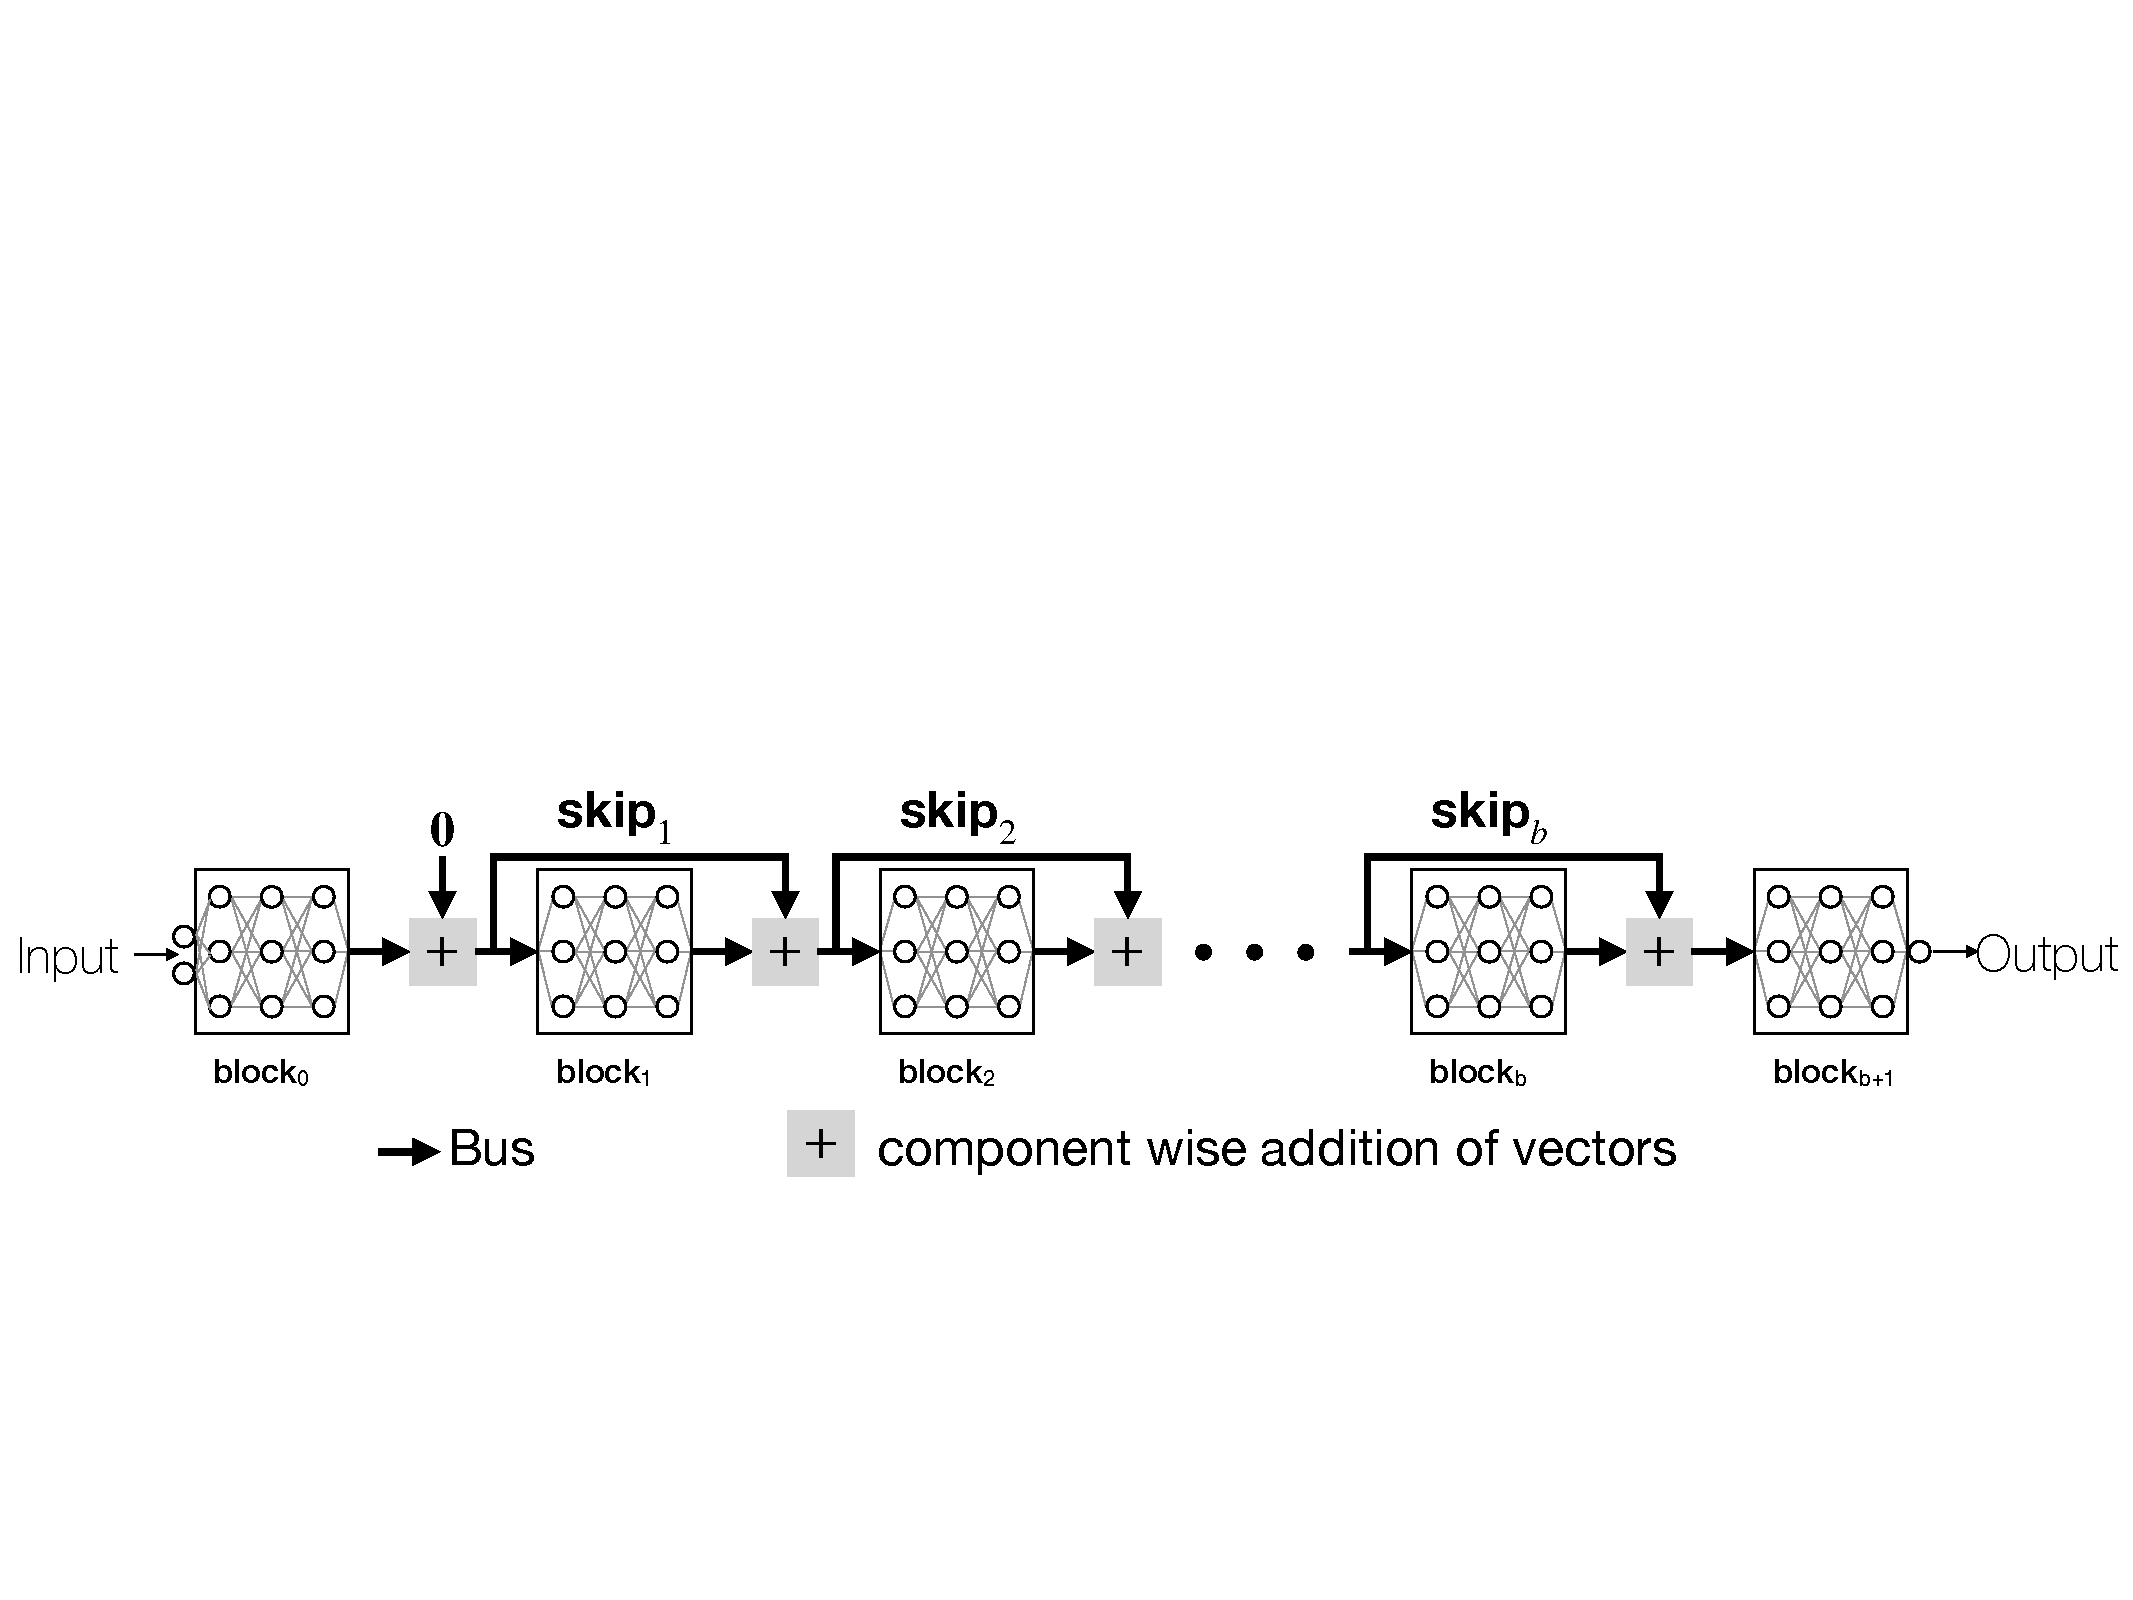
\includegraphics[scale=0.5]{figs/resnet.pdf}
}
\end{minipage}
\begin{minipage}{0.5\columnwidth}
\resizebox{\columnwidth}{!}{
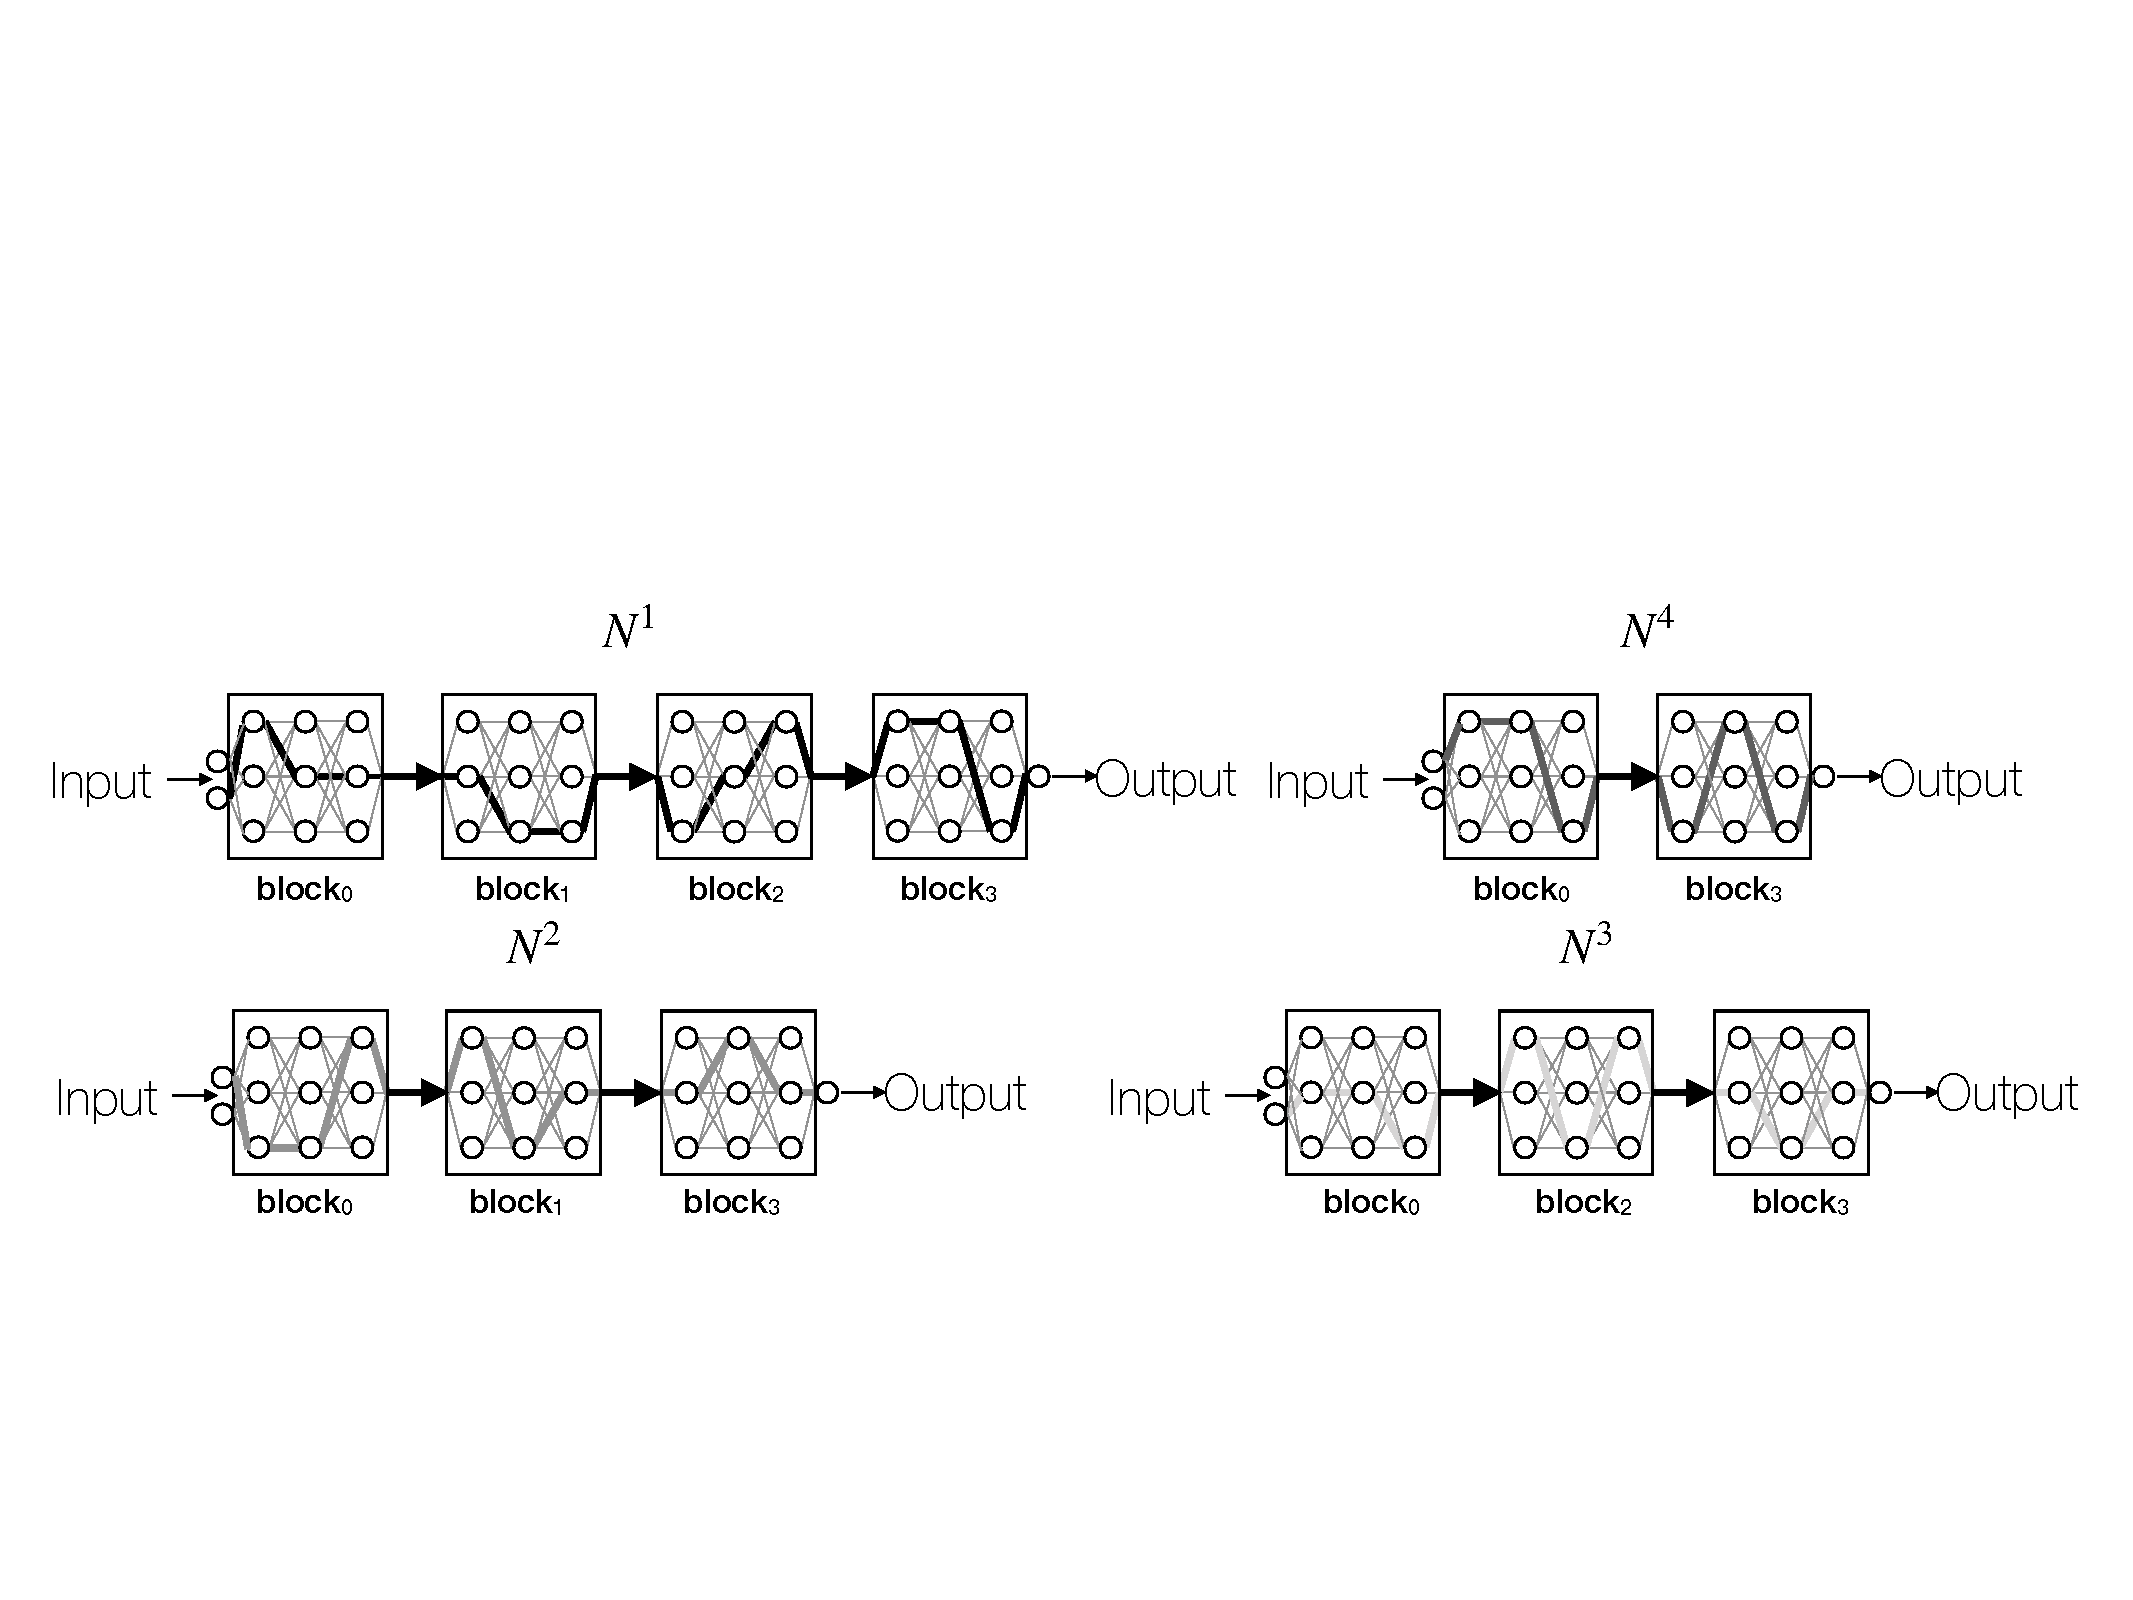
\includegraphics[scale=0.5]{figs/blocks.pdf}
}
\end{minipage}
\caption{\small{On the left is the ResNet with $b$ skip connections and $(b+2)$ blocks. On the right are the sub-FC networks $N^1$ obtained by skipping no blocks, $N^2$ and $N^4$ obtained by skipping block $1$ and $2$ respectively, and $N^3$ obtained by skipping both blocks $1$ and $2$.}}
\label{fig:resnet}
\end{figure}

\begin{definition}\label{def:subfcdnn}[Sub FC-DNNs]
Let $2^{[b]}$ denote the power set of $[b]$ and let $\J\in 2^{[b]}$ denote any subset of $[b]$. Define the`$\J^{th}$' sub-FC-DNN of the ResNet to be the fully connected network obtained by (i) including  $\text{block}_{j},\forall j\in \J$  and (ii) ignoring $\text{block}_{j},\forall j\notin \J$ (see \Cref{fig:resnet}).
\end{definition}
\begin{theorem}
[Sum of Product of Kernels Theorem]\label{th:res} Let $\text{NPK}^{\J}$ be the NPK of the $\J^{th}$ sub-FC-DNN, and $\bfc^{\J}$ be the associated constant. Under \Cref{assmp:main}, we have:
\begin{align*}
\text{NTK}\rightarrow \sum_{\J\in 2^{[b]}}  \bfc^{\J} \text{NPK}^{\J}, \,\, \text{as}\,\,  w\rightarrow\infty
\end{align*}
\end{theorem}
\textbf{Note.} The sub-FC-DNNs we refer to in \Cref{th:mainres} belong to (or are parts of) the feature network from which the gates are obtained. 

$\bullet$  In \Cref{th:fc} is mathematically equivalent to Theorem 5.1 in \citep{npk} (stated as \Cref{th:fcprev}). The equivalence follows from the simple observation that $\textbf{overlap}(x,x')=\Pi_{l=1}^{(d-1)}\ip{G_l(x),G_l(x')}$. %To see this, for sake of simplicity, consider, say a network with $d=3$ layers, and for both inputs $x,x'$, say $5$ gates are active in the first layer and $4$ gates are active in the second layer, then $\textbf{overalp}(x,x')=20=\ip{G_1(x),G_1(x')}\times \ip{G_2(x),G_2(x')}= 5\times 4$ is . Now, if we interchange the layers, then we will have again $\textbf{overalp}(x,x')= 20=\ip{G_2(x),G_2(x')}\times \ip{G_1(x),G_1(x')}=4\times 5$. 
While this observation is very elementary in itself, it is significant at the same time; in \Cref{th:fc} it provides the most simplest kernel expression that characterises the information in the gates. It also explains the roles of width and depth. From \Cref{th:fc} it is evident that the role of width is \emph{averaging} (due to the division by $w$). Each layer therefore corresponds to a \emph{base kernel} $\frac{\ip{G_l(x),G_l(x')}}w$ which measures the \emph{\textbf{correlation of the gates}}. The role of depth is to provide the product of kernels. To elaborate, the feature network provides the layer-by-layer gating information, and the value network implements the product of kernels by laying out the gates as masks depth-wise, and connecting them in the structure of a deep network. Note that depth-wise layout plays an important role here: for instance, if we were to concatenate the gating features as $\varphi(x)=(G_l(x),l=1,\ldots,d-1)\in\{0,1\}^{(d-1)w}$, it would have only resulted in the kernel $\ip{\varphi(x),\varphi(x')}=\sum_{l=1}^{d-1}{\ip{G_l(x),G_l(x')}}$, i.e., a \emph{sum  (not product)} of kernels. 

$\bullet$ \Cref{th:conv}: $\sum_{r=0}^{\din-1} \ip{x,rot(x',r)}_{\Lambda(\cdot, x,rot(x',r))}=\sum_{r=0}^{\din-1} \left(\sum_{i=1}^{\din} x(i) rot(x',r)(i)\Lambda(i,x,x')\right)$, where the inner `$\Sigma$' is the inner product between $x$ and $rot(x',r)$ weighted by $\Lambda$ and the outer `$\Sigma$' covers all possible rotations, which results in the rotational invariance property. The rotational invariance property holds for architectures using convolutional layer only in the presence of global-pooling. It was observed in the experiments of \cite{arora2019exact} that networks with global-average-pooling are better than vanilla convolutional networks. That said, the rotational invariance property of the kernel is not a new observation in this paper; it was shown by \cite{li2019enhanced} that  prediction using CNTK-GAP is equivalent to prediction using CNTK without GAP but with full translation data augmentation with wrap-around at the boundary. However, \Cref{th:conv} is a necessary result, in that, it demonstrates that this rotational invariance property is recovered in the dual view as well. We also note here that the rotational invariance property continues to hold even if we provide a constant $\mathbf{1}$ input and also destroy the layer-by-layer structure, which are novel insights that naturally follow from the dual path-by-path formulation.

$\bullet$ \Cref{th:res} shows that skip connections give rise to an ensemble kernel (sum of many kernels). Specifically, each kernel in the ensemble, i.e., $\text{NPK}^{\J}$ corresponds to one of the $2^b$ sub-architectures (see \Cref{def:subfcdnn}). The ensemble behaviour of ResNet and  presence of $2^b$ architectures was observed by \cite{veit2016residual}. They showed that  ``removing single layers from residual networks at test time does not noticeably affect their performance", and yet ``removing a layer from a traditional architecture such as VGG [18] leads to a dramatic loss in performance". In other words, due to the ensemble structure a ResNet is capable of dealing with failure of components. While, failure of component itself does not occur unless one makes them fail purposefully in experiments as done in \citep{veit2016residual},  the way to look at failure is to think that one or many of the kernels in the ensemble are corrupt and the good ones are compensating for them. The main novelty in our paper compared to \citep{veit2016residual} is that we provide a mathematical framework and also the expression for the ensemble kernel. Thus, our results are theoretical and \citep{veit2016residual} presents empirical results without rigorous theory.

%In order to completely address the `black box'-ness issue, an ideal goal is to aim for theoretical results (supported by empirical evidence) on finite time learning in finite width \texttt{DGN-NO-ACT}. We find this goal is too hard at this stage and do not pursue the same. The next level is to analyse  the primal linearity and the dual linearity separately. Understanding the primal linearity has two parts to it (i) `what do the learnt pre-activations mean?', and (ii) `how are useful pre-activations learnt?'. The `what' question is \emph{post-hoc}, i.e., we can inspect the learnt pre-activations after training. However, we believe that in order to obtain domain specific insights on what the learnt pre-activations mean, we might require domain specific tools. For instance, in the case of `image classification', the pre-activations are the result of series of convolutions by `filter banks', and in order to do full justice, any visual interpretation should also tally with the results from `filter bank' theory. We defer the `what' question for future work. We also believe new theory is required to answer `how are useful pre-activations learnt?', and defer the same to future work. In this paper,  


%$\bullet$ We empirically show that \texttt{DGN-NO-ACT} performs comparably well on standard datasets. 

%$\bullet$ We restate the prior result for the fully connected case so as to explicitise the role of gates, depth and width. We extend the dual view theory to cover  convolutions with global pooling and skip connections.  We show empirically that the value network learns path-by-path and not layer-by-layer.




%A \texttt{DGN-NO-ACT} learns the relation $\hat{y}(x)=\ip{\phi_\Tf(x),v_{\Tv}}$, by learning simultaneously the feature and value network parameters. The pre-activations generated by the feature network trigger the gates thereby directly dictating the neural path feature $\phi_\Tf(x)$. It was shown that neural path features (i.e., the gates) are learnt during training and such learning improves generalisation \cite{npk}. Thus, while the learning in feature network is key, we reserve its theoretical study for future work. In this section, we will analyse the dual linearity, wherein, the theoretical results are in the \emph{inifinite width regime} which yield us a \emph{kernel} interperation, using which we probe into the properties of finite width networks. In other words, our aim is not to propose pure kernel methods with the kernel derived from an inifnite width DNN. 

%For the purpose of analysing the dual, we first explicitise in \Cref{th:fc} an unnoticed invariance property in the prior result of \cite{npk} for fully connected networks. In \Cref{th:conv,th:res} we also extend the dual formulation to cover the cases of convolutions with global pooling and skip connections. These results justify the constant $\mathbf{1}$ input to the value network of the \texttt{DGN-NO-ACT}. We also experimentally verify the constant $\mathbf{1}$ input as well as destroying the layer-by-layer structure of the gates does not degrade the performance. While these results are surprising and counter intuitive with respect to the primal view, they are follow in a straightforward manner from the results in the dual view, thereby underscoring the fact the value network indeeed computes path-by-path, and eliminating the `mystery' as to whether sophisticated structures are learnt layer-by-layer.


\begin{figure}
\centering
\begin{minipage}{1.0\columnwidth}
\centering
\begin{minipage}{0.49\columnwidth}
\resizebox{0.99\columnwidth}{!}{
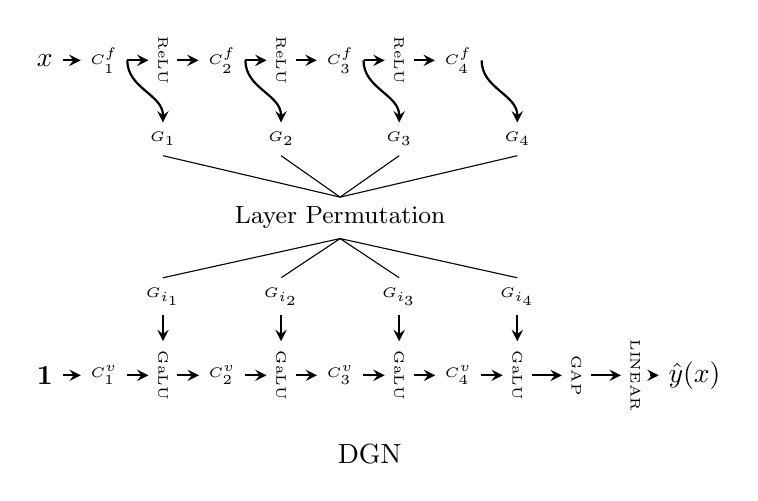
\begin{tikzpicture}
%%%%%%%%%%%%%%%%%%%%%%%%%%%%%%%%%%%%%%%%%%%%%%%%%%%%%%%%%%%%%%%%%
\node []  (fntext)at (4.625,-3.5) {DGN};

%\node []  (output) at (7.5,1.5) {$\hat{y}(x)$};


\node [] (dgn-f-c4) at (5.75,1.5){\tiny{$C^{\text{f}}_4$}};


\node [rotate=-90] (dgn-relu-3) at (5,1.5){\tiny{ReLU}};
\node [] (dgn-f-c3) at (4.25,1.5){\tiny{$C^{\text{f}}_3$}};
\draw [-stealth,thick]   (dgn-f-c3.east) -- (dgn-relu-3.south);
\draw [-stealth,thick]   (dgn-relu-3.north) -- (dgn-f-c4.west);


\node [rotate=-90] (dgn-relu-2) at (3.5,1.5){\tiny{ReLU}};
\node [] (dgn-f-c2) at (2.75,1.5){\tiny{$C^{\text{f}}_2$}};
\draw [-stealth,thick]   (dgn-f-c2.east) -- (dgn-relu-2.south);
\draw [-stealth,thick]   (dgn-relu-2.north) -- (dgn-f-c3.west);


\node [rotate=-90] (dgn-relu-1) at (2,1.5){\tiny{ReLU}};
\node [] (dgn-f-c1) at (1.25,1.5){\tiny{$C^{\text{f}}_1$}};
\draw [-stealth,thick]   (dgn-f-c1.east) -- (dgn-relu-1.south);
\draw [-stealth,thick]   (dgn-relu-1.north) -- (dgn-f-c2.west);



\node [] (dgn-f-input) at (0.5,1.5){$x$};
\draw [-stealth,thick]   (dgn-f-input.east) -- (dgn-f-c1.west);




\node []  (dgn-output) at (8.75,-2.5) {$\hat{y}(x)$};
\node [rotate=-90] (dgn-smax) at (8,-2.5){\tiny{LINEAR}};
\draw [-stealth,thick]   (dgn-smax.north)--(dgn-output.west);

\node [rotate=-90] (dgn-gap) at (7.25,-2.5){\tiny{GAP}};
\draw [-stealth,thick]   (dgn-gap.north)--(dgn-smax.south);



\node [rotate=-90] (dgn-galu-4) at (6.5,-2.5){\tiny{GaLU}};
\draw [-stealth,thick]   (dgn-galu-4.north) -- (dgn-gap.south);

\node [] (dgn-v-c4) at (5.75,-2.5){\tiny{$C^{\text{v}}_4$}};
\draw [-stealth,thick]   (dgn-v-c4.east) -- (dgn-galu-4.south);

\node [rotate=-90] (dgn-galu-3) at (5,-2.5){\tiny{GaLU}};
\node [] (dgn-v-c3) at (4.25,-2.5){\tiny{$C^{\text{v}}_3$}};
\draw [-stealth,thick]   (dgn-v-c3.east) -- (dgn-galu-3.south);
\draw [-stealth,thick]   (dgn-galu-3.north) -- (dgn-v-c4.west);



\node [rotate=-90] (dgn-galu-2) at (3.5,-2.5){\tiny{GaLU}};
\node [] (dgn-v-c2) at (2.75,-2.5){\tiny{$C^{\text{v}}_2$}};
\draw [-stealth,thick]   (dgn-v-c2.east) -- (dgn-galu-2.south);
\draw [-stealth,thick]   (dgn-galu-2.north) -- (dgn-v-c3.west);


\node [rotate=-90] (dgn-galu-1) at (2,-2.5){\tiny{GaLU}};
\node [] (dgn-v-c1) at (1.25,-2.5){\tiny{$C^{\text{v}}_1$}};

\draw [-stealth,thick]   (dgn-v-c1.east) -- (dgn-galu-1.south);
\draw [-stealth,thick]   (dgn-galu-1.north) -- (dgn-v-c2.west);




\node [] (dgn-input) at (0.5,-2.5){$\mathbf{1}$};
\draw [-stealth,thick]   (dgn-input.east) -- (dgn-v-c1.west);


\node[] (dgn-gating-1-up) at (2,0.5){\tiny{$G_{1}$}};
\draw [-stealth,thick]   (dgn-f-c1.east) to[out=-90,in=90] (dgn-gating-1-up.north);


\node[] (dgn-gating-2-up) at (3.5,0.5){\tiny{$G_{2}$}};
\draw [-stealth,thick]   (dgn-f-c2.east) to[out=-90,in=90] (dgn-gating-2-up.north);



\node[] (dgn-gating-3-up) at (5,0.5){\tiny{$G_{3}$}};
\draw [-stealth,thick]   (dgn-f-c3.east) to[out=-90,in=90] (dgn-gating-3-up.north);


\node[] (dgn-gating-4-up) at (6.5,0.5){\tiny{$G_{4}$}};
\draw [-stealth,thick]   (dgn-f-c4.east) to[out=-90,in=90] (dgn-gating-4-up.north);





\node[] (dgn-gating-1) at (2,-1.5){\tiny{$G_{i_1}$}};
\draw [-stealth,thick]   (dgn-gating-1.south) -- (dgn-galu-1.west);


\node[] (dgn-gating-2) at (3.5,-1.5){\tiny{$G_{i_2}$}};
\draw [-stealth,thick]   (dgn-gating-2.south) -- (dgn-galu-2.west);



\node[] (dgn-gating-3) at (5,-1.5){\tiny{$G_{i_3}$}};
\draw [-stealth,thick]   (dgn-gating-3.south) -- (dgn-galu-3.west);


\node[] (dgn-gating-4) at (6.5,-1.5){\tiny{$G_{i_4}$}};
\draw [-stealth,thick]   (dgn-gating-4.south) -- (dgn-galu-4.west);



\node[] (permutation) at (4.25,-0.5){\small{Layer Permutation}};

\draw [-]   (dgn-gating-1-up.south) -- (permutation.north);
\draw [-]   (dgn-gating-4-up.south) -- (permutation.north);
\draw [-]   (dgn-gating-2-up.south) -- (permutation.north);
\draw [-]   (dgn-gating-3-up.south) -- (permutation.north);



\draw [-]  (permutation.south) --  (dgn-gating-1.north)  ;
\draw [-]  (permutation.south) --  (dgn-gating-2.north)  ;
\draw [-]  (permutation.south) --  (dgn-gating-3.north)  ;
\draw [-]  (permutation.south) --  (dgn-gating-4.north)  ;

	
\end{tikzpicture}


}
\end{minipage}
\begin{minipage}{0.49\columnwidth}
\resizebox{0.99\columnwidth}{!}{
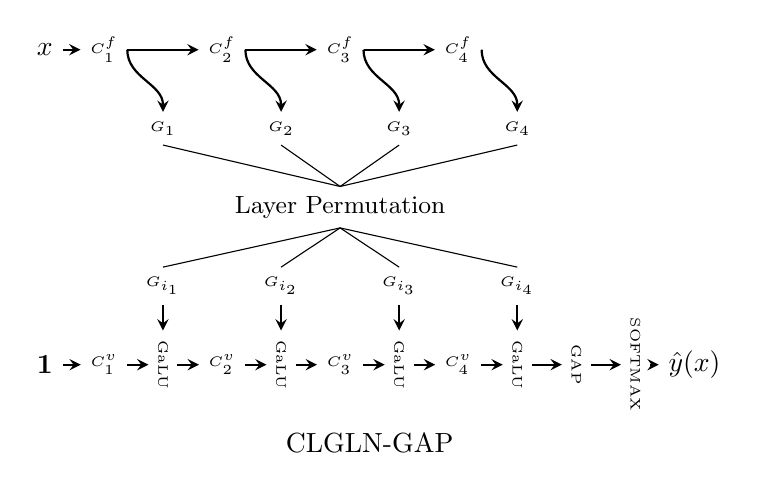
\begin{tikzpicture}
\node []  (fntext)at (-4.625,-3.5) {CLGLN-GAP};

%\node []  (output) at (7.5,1.5) {$\hat{y}(x)$};


\node [] (dgn1-f-c4) at (-3.5,1.5){\tiny{$C^{\text{f}}_4$}};
\node [] (dgn1-f-c3) at (-5,1.5){\tiny{$C^{\text{f}}_3$}};
\node [] (dgn1-f-c2) at (-6.5,1.5){\tiny{$C^{\text{f}}_2$}};
\node [] (dgn1-f-c1) at (-8,1.5){\tiny{$C^{\text{f}}_1$}};
\node [] (dgn1-input-f) at (-8.75,1.5){$x$};
\draw [-stealth,thick]   (dgn1-f-c3.east) -- (dgn1-f-c4.west);
\draw [-stealth,thick]   (dgn1-f-c2.east) -- (dgn1-f-c3.west);
\draw [-stealth,thick]   (dgn1-f-c1.east) -- (dgn1-f-c2.west);
\draw [-stealth,thick]   (dgn1-input-f.east) -- (dgn1-f-c1.west);



\node []  (dgn1-output) at (-0.5,-2.5) {$\hat{y}(x)$};

\node [rotate=-90] (dgn1-smax) at (-1.25,-2.5){\tiny{SOFTMAX}};
\draw [-stealth,thick]   (dgn1-smax.north)--(dgn1-output.west);

\node [rotate=-90] (dgn1-gap) at (-2,-2.5){\tiny{GAP}};
\draw [-stealth,thick]   (dgn1-gap.north)--(dgn1-smax.south);


\node [rotate=-90] (dgn1-galu-4) at (-2.75,-2.5){\tiny{GaLU}};
\draw [-stealth,thick]   (dgn1-galu-4.north)--(dgn1-gap.south);

\node [] (dgn1-v-c4) at (-3.5,-2.5){\tiny{$C^{\text{v}}_4$}};
\draw [-stealth,thick]   (dgn1-v-c4.east) -- (dgn1-galu-4.south);


\node [rotate=-90] (dgn1-galu-3) at (-4.25,-2.5){\tiny{GaLU}};
\draw [-stealth,thick]   (dgn1-galu-3.north) -- (dgn1-v-c4.west);

\node [] (dgn1-v-c3) at (-5,-2.5){\tiny{$C^{\text{v}}_3$}};
\draw [-stealth,thick]   (dgn1-v-c3.east) -- (dgn1-galu-3.south);


\node [rotate=-90] (dgn1-galu-2) at (-5.75,-2.5){\tiny{GaLU}};
\draw [-stealth,thick]   (dgn1-galu-2.north) -- (dgn1-v-c3.west);

\node [] (dgn1-v-c2) at (-6.5,-2.5){\tiny{$C^{\text{v}}_2$}};
\draw [-stealth,thick]   (dgn1-v-c2.east) -- (dgn1-galu-2.south);


\node [rotate=-90] (dgn1-galu-1) at (-7.25,-2.5){\tiny{GaLU}};
\draw [-stealth,thick]   (dgn1-galu-1.north) -- (dgn1-v-c2.west);


\node [] (dgn1-v-c1) at (-8,-2.5){\tiny{$C^{\text{v}}_1$}};
\draw [-stealth,thick]   (dgn1-v-c1.east) -- (dgn1-galu-1.south);


\node [] (dgn1-v-input) at (-8.75,-2.5){$\mathbf{1}$};

\draw [-stealth,thick]   (dgn1-v-input.east) -- (dgn1-v-c1.west);


\node[] (dgn1-gating-4-up) at (-2.75,0.5){\tiny{$G_{4}$}};
\draw [-stealth,thick]   (dgn1-f-c4.east) to[out=-90,in=90] (dgn1-gating-4-up.north);


\node[] (dgn1-gating-3-up) at (-4.25,0.5){\tiny{$G_{3}$}};
\draw [-stealth,thick]   (dgn1-f-c3.east) to[out=-90,in=90] (dgn1-gating-3-up.north);



\node[] (dgn1-gating-2-up) at (-5.75,0.5){\tiny{$G_{2}$}};
\draw [-stealth,thick]   (dgn1-f-c2.east) to[out=-90,in=90] (dgn1-gating-2-up.north);


\node[] (dgn1-gating-1-up) at (-7.25,0.5){\tiny{$G_{1}$}};
\draw [-stealth,thick]   (dgn1-f-c1.east) to[out=-90,in=90] (dgn1-gating-1-up.north);





\node[] (dgn1-gating-4) at (-2.75,-1.5){\tiny{$G_{i_4}$}};
\draw [-stealth,thick]   (dgn1-gating-4.south) -- (dgn1-galu-4.west);


\node[] (dgn1-gating-3) at (-4.25,-1.5){\tiny{$G_{i_3}$}};
\draw [-stealth,thick]   (dgn1-gating-3.south) -- (dgn1-galu-3.west);



\node[] (dgn1-gating-2) at (-5.75,-1.5){\tiny{$G_{i_2}$}};
\draw [-stealth,thick]   (dgn1-gating-2.south) -- (dgn1-galu-2.west);


\node[] (dgn1-gating-1) at (-7.25,-1.5){\tiny{$G_{i_1}$}};
\draw [-stealth,thick]   (dgn1-gating-1.south) -- (dgn1-galu-1.west);



\node[] (permutation1) at (-5,-0.5){\small{Layer Permutation}};

\draw [-]   (dgn1-gating-1-up.south) -- (permutation1.north);
\draw [-]   (dgn1-gating-4-up.south) -- (permutation1.north);
\draw [-]   (dgn1-gating-2-up.south) -- (permutation1.north);
\draw [-]   (dgn1-gating-3-up.south) -- (permutation1.north);



\draw [-]  (permutation1.south) --  (dgn1-gating-1.north)  ;
\draw [-]  (permutation1.south) --  (dgn1-gating-2.north)  ;
\draw [-]  (permutation1.south) --  (dgn1-gating-3.north)  ;
\draw [-]  (permutation1.south) --  (dgn1-gating-4.north)  ;


%%%%%%%%%%%%%%%%%%%%%%%%%%%%%%%%%%%%%%%%%%%%%%%%%%%%%%%%%%%%%%%%%

	
\end{tikzpicture}


}
\end{minipage}
\end{minipage}
\caption{$4$ convolutional layers with GAP}
\label{fig:c4gap}
\end{figure}

\begin{table}
\centering
\begin{tabular}{ccccccc}
\toprule 
Dataset & Model & DNN & DGN$(x,x)$ & DGN$(x,\mathbf{1})$ &  LGLN$(x,x)$ & LGLN$(x,\mathbf{1})$\\\midrule
\multirow{3}{*}{CIFAR10}& C4GAP & DNN & DGN$(x,x)$ & DGN$(x,\mathbf{1})$ &  LGLN$(x,x)$ & LGLN$(x,\mathbf{1})$\\
& VGG16-AP & DNN & DGN$(x,x)$ & DGN$(x,\mathbf{1})$ &  LGLN$(x,x)$ & LGLN$(x,\mathbf{1})$\\
&ResNet110 & DNN & DGN$(x,x)$ & DGN$(x,\mathbf{1})$ &  LGLN$(x,x)$ & LGLN$(x,\mathbf{1})$\\\midrule
\multirow{2}{*}{CIFAR100} & VGG16-AP & DNN & DGN$(x,x)$ & DGN$(x,\mathbf{1})$ &  LGLN$(x,x)$ & LGLN$(x,\mathbf{1})$\\
&ResNet110 & DNN & DGN$(x,x)$ & DGN$(x,\mathbf{1})$ &  LGLN$(x,x)$ & LGLN$(x,\mathbf{1})$\\

\bottomrule
\end{tabular}
\caption{Summary of Experiments}
\label{tb:expresults}
\end{table}



